\section{Closeness Centrality in Street Network Analysis}\label{closeness_centrality}

\subsection{Varying descriptions for the concept of closeness}

Application of the concept of closeness to street network analysis emerged with the development of space syntax in the late 1970s and early 1980s \cite{Hillier1984}. In this context, closeness is referred to as \emph{Integration} and implies ``to-movement'' or ``closeness'' in the general sense of the words \footnote{We here and throughout the paper refer to uncapitalised ``closeness'' in the general sense, as opposed to the capitalised form which we use to express the formal mathematical definition for \emph{Closeness}, a specific form of closeness centrality.}. In the case of the axial topological network representations used at the time, \emph{Integration} is calculated through counting the number of topological steps to surrounding nodes, taking the average, ``relativising'' the result to the size of the network, then taking the reciprocal, thereby converting the measure from farness-like to closeness-like.

After the introduction and increasing shift to angular segment analysis in the 2000s, which used street segments based on road centrelines instead of axial lines, the method for calculating \emph{Integration} was adapted to work with weighted graph edges by using summed angular deviation instead of counting topological steps. Whereas Turner at first suggested the use of \emph{Normalised Closeness} (Equation~\ref{eq:normalised_closeness}) \cite{Turner2007}, he would later suggest taking the node count divided by the average distance to the nodes \cite{turner_getting_2008}, which reflects the same intention as with the aforementioned axial integration: take \emph{Normalised Farness} (average distance), re-normalise by the number of nodes in the network, then take the reciprocal. This is reinforced in a subsequent paper \cite{Hillier2012}, where Hillier and Turner et al.\ state that the Depthmap software package calculates angular segment integration by \emph{``dividing mean angular depth by node count... and taking the reciprocal''} (where \emph{Mean Depth} refers to average distance). Closer inspection shows that this variant of closeness resembles a simplified form of the so-called \emph{Improved Closeness} (see Equations~\ref{eq:improved_closeness},~\ref{eq:used_closeness}) proposed by Wasserman and Faust \cite{Wasserman1994}, which differs from \emph{Normalised Closeness} in that it divides the node count by the \textbf{average} as opposed to \textbf{total} distance to the nodes. Notably, at least three street network analysis packages continue to use or provide this form of \emph{Improved Closeness}, including \texttt{Depthmap} \cite{Hillier2012, turner_depthmapx_2020}, the \texttt{Place Syntax Tool} \cite{stahle_place_2023}, and the \texttt{cityseer} Python package \cite{simons_cityseer_2023}.

Concurrent with the adoption of road centreline representations in the mid-2000s, and the wider interest in street network analysis more generally, researchers both within and outside of space syntax have since consistently cited \emph{Normalised Closeness} (Equation~\ref{eq:normalised_closeness}) when referring to the measure of closeness, even when these citations depend on packages such as \texttt{Depthmap} \cite{Omer2018}. Citations for non-normalised mathematical \emph{Closeness} (Equation~\ref{eq:closeness}) and even \emph{Normalised Farness} (Equation~\ref{eq:normalised_farness}) are also found. We present a selection of example references in Table~\ref{table:closeness_literature}.

\begin{table}[htbp]
  \centering

  \begin{tabular}{p{3.5cm} p{11cm}}
    \toprule
    \emph{Closeness} \& \emph{Normalised Closeness} & Representative of literature citations on street network analysis in general, which typically mention or show the formula for \emph{Normalised Closeness} \cite{crucitti_centrality_2006, Porta2009, Masucci2016, vaughan_glossary_2025, Turner2007, noauthor_segment_nodate, Porta2006} though also often discussed in the non-normalised form \cite{hutchison_network_2005, Sevtsuk2012, Cooper2015, Batty2013}. \\

    \midrule
    \emph{Improved Closeness} & Limited examples, which tend to come from technical literature or street network analysis computational packages \cite{turner_depthmapx_2020, stahle_place_2023, simons_cityseer_2023}. This form divides the node count by the \textbf{average} as opposed to \textbf{total} distance to the nodes. \\
    & \emph{``Hillier has suggested $Integ = NC / MD$ where NC is node count (i.e., the number of nodes within a network radius), and MD is mean depth of the nodes with respect to the root node.'' \cite{turner_getting_2008}} \\
    & \emph{``Angular segment analysis: The integration solution. Hillier's integration measure gives a solution that works both at low radius and radius n: $Integ = (NC * NC) / TD$'' \cite{turner_getting_2008}} (Algebraically rearranged form of $Integ = NC / MD$). \\
    & \emph{``...the current angular integration measure in Depthmap. This is found by re-dividing mean angular depth by node count... and taking the reciprocal to have high values for high integration'' \cite{Hillier2012}} \\

    \midrule
    \emph{Normalised Farness} & Limited examples, which possibly unintentionally omit mention of taking the reciprocal (which would then give \emph{Normalised Closeness}). \\
    & \emph{``Segment integration / segment angular closeness of a segment is the mean of all the angles of all the shortest paths...'' ($C_\theta$) \cite{rashid_geometry_2017, van_nes_introduction_2021}} \\
    & \emph{``Closeness...calculates the average distance from each node to all other nodes...'' \cite{Gil2017}} \\
    \bottomrule
  \end{tabular}

  \captionof{table}{Examples of different formulations attributed to the concept of closeness.}
  \label{table:closeness_literature}
\end{table}

\subsection{Research Question}

The context of our research question stems from the varying cited definitions of closeness centralities for street network analysis. At first glance, this may simply be attributable to historical evolution or different traditions of analysis; however, closer scrutiny is warranted given the divergence between cited formulations and those used by several computational packages. This has potentially significant ramifications for the comparability of findings and the reproducibility of results.

We accordingly ask whether there is a distinction in the behaviour of \emph{Improved Closeness} and \emph{Normalised Closeness} in the context of contemporary street network analysis. By ``contemporary'', we imply the use of either \emph{metric distances} (in metres) or \emph{geometric distances} (in angular deviation) on networks constructed from topologically cleaned road centreline representations, and where the measures are computed using localised methods to control for edge effects, thereby facilitating comparisons across locations and scales of analysis (see Section~\ref{network-analysis}).

We proceed with a theoretical hypothesis for why a distinction between \emph{Improved Closeness} and \emph{Normalised Closeness} is potentially meaningful for closeness centralities in street network analysis. We then conduct an empirical evaluation where we compare the behaviour of different forms of closeness centrality in the context of landuse and trip data to confirm whether the measures behave as anticipated by the hypothesis.

\subsection{Hypothesis}

As discussed in Section~\ref{network-analysis}, complications with boundary edge effects means that street network analysis has shifted to using distance localised sub-graphs for comparability across locations and scales of analysis. Turner, an early developer of road centreline street network analysis methods, expresses in a presentation given in 2008 that they (including Bill Hillier) were looking for a closeness-like formulation that is compatible with localised methods of analysis, for which a form of \emph{Improved Closeness} is proposed \cite{turner_getting_2008} (see quotations in Table~\ref{table:closeness_literature}) and subsequently adopted into \texttt{depthmap} \cite{Hillier2012}. Other than for developers of computational packages, we surmise that the distinction on workable formulations for localised closeness analysis appears not to have been broadly recognised by the wider street network analysis research community, where literature now almost universally refers to \emph{Normalised Closeness} even in the context of the predominantly used localised methods. We consequently hypothesise that \emph{Normalised Closeness} may produce counter-intuitive results for localised forms of network analysis and proceed with a theoretical description for why this may be the case.

When formally defined, the mathematical \emph{Closeness} measure
\begin{equation}\label{eq:closeness}
  Closeness_{(i)} = \frac{1}{\sum_{j\neq{i}}d_{(i,j)}}
\end{equation}
is the reciprocal of \emph{farness}
\begin{equation}\label{eq:farness}
  Farness_{(i)} = \sum_{j\neq{i}}d_{(i,j)}\, ,
\end{equation}
where \emph{Farness} is the sum of distances $d$ from node $i$ to all reachable nodes $j$ \cite{Sabidussi1966}. Mathematical \emph{Closeness} conveys how proximate node $i$ is to surrounding nodes, with the implication that high closeness centralities afford increased likelihood of access and interaction. \emph{Closeness} can be normalised by the number of nodes in the graph $N$ divided by the sum of the distances
\begin{equation}\label{eq:normalised_closeness}
  Normalised\ Closeness_{(i)} = \frac{N-1}{\sum_{j\neq{i}}d_{(i,j)}}\ ,
\end{equation}
which is the inverse of the arithmetic mean (average) of \emph{Farness}:
\begin{equation}\label{eq:normalised_farness}
  Normalised\ Farness_{(i)} = \frac{\sum_{j\neq{i}}d_{(i,j)}}{N-1}\ .
\end{equation}
When normalising, it is common to use $N-1$ to imply that the origin node $i$ is not technically counted (though this only has a notable impact on small graphs).

In the broader network analysis field, it has been shown that \emph{Harmonic Closeness} centrality \cite{Marchiori2000, Rochat2009} scales more reliably for disconnected sub-graphs, with the difference being that the division happens prior to the summation
\begin{equation}\label{eq:harmonic_closeness}
  Harmonic\ Closeness_{(i)} = \sum_{j\neq{i}}\frac{1}{d_{(i,j)}}\ .
\end{equation}

For the same reason, others have suggested \emph{Improved Closeness} centrality \cite{Wasserman1994}
\begin{equation}\label{eq:improved_closeness}
  Improved\ Closeness_{(i)} = \frac{N_{i}/{g}}{\sum_{j\neq{i}}d_{(i,j)}/{N_{i}}}\, ,
\end{equation}
which is intended for situations where a limited subset of nodes is reachable. It is defined as the ratio of the fraction of reachable nodes $N_{i}/{g}$ to the average distance to those nodes $\sum_{j\neq{i}}d_{(i,j)}/{N_{i}}$. In the context of street network analysis, the global number of nodes $g$ is ordinarily unknown; nevertheless, since this is effectively the worldwide street network and is constant for all sub-graphs, it can be proposed that the number of reachable nodes $N_{i}$ in the numerator can forego the normalisation by $g$, thus giving
\begin{equation}\label{eq:used_closeness}
  Improved\ Closeness_{(i)} = \frac{N_{i}}{\sum_{j\neq{i}}d_{(i,j)}/{N_{i}}} = \frac{N_{i}^2}{\sum_{j\neq{i}}d_{(i,j)}}\ ,
\end{equation}
which is synonymous with the formula proposed by Turner and Hillier and the variant found in several computational packages. (Note that when algebraically rearranged, the formulation can be expressed as the square of the number of reachable nodes divided by the sum of the distances to those nodes.)

The intuition of \emph{Improved Closeness} can be contrasted to \emph{Normalised Closeness} (Eq:~\ref{eq:normalised_closeness}): the number of reachable nodes is divided by the \textbf{average} distance instead of the \textbf{total} distance to the nodes. This distinction is important for localised graphs because \emph{Improved Closeness} is consequently able to scale intuitively even if the number of nodes varies: it increases either for a greater number of locally accessible nodes or if the average distance to those nodes decreases.

Figure~\ref{fig:closeness_comparisons} illustrates the implications with a simple example: Scenario B is expected to have greater closeness within an urban context than Scenario A because it is equivalently close to a greater number of nodes. Scenario C contains a more distant node and should therefore have a lower closeness centrality than Scenario B but should still be greater than A.

\begin{figure}[htbp]
  \centering
  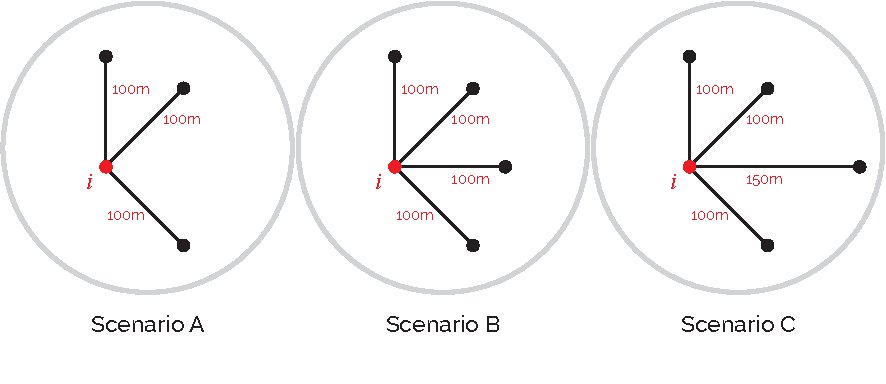
\includegraphics[width=\linewidth, keepaspectratio]{images/closeness_comparisons.pdf}
  \caption{Simple comparative localised closeness scenarios.}\label{fig:closeness_comparisons}
\end{figure}

As shown in Table~\ref{table:closeness_comparisons}, in the context of localised analysis, mathematical \emph{Closeness} behaves opposite to its intended usage because it scales differently across different quantities of nodes, decreasing from Scenario A to B and from A to C. This means that whereas mathematical \emph{Closeness} may be useful for comparing the centralities of nodes within the same graph, it behaves counter-intuitively when comparing centralities across graphs containing different numbers of nodes. \emph{Normalised Closeness} is similarly problematic for localised analysis because it now neutralises meaningful variations, such as from Scenario A to B, while also continuing to demonstrate unexpected behaviour, such as counter-intuitively decreasing from Scenario A to C. On the other hand, and as indicated in the broader network analysis literature, \emph{Harmonic Closeness} \cite{Rochat2009} and the simplified form of \emph{Improved Closeness} \cite{Wasserman1994} behave in a manner consistent with expectations across differently sized sub-graphs.

\begin{table*}[htbp]
  \centering
  \begin{tabular}{ r | r r r }
    &
    Scenario A &
    Scenario B &
    Scenario C \\
    \midrule
    \\
    $Closeness$ &
    $\frac{1}{100+100+100}=0.00\overline{3}$ &
    $\frac{1}{100+100+100+100}=0.0025$ &
    $\frac{1}{100+100+150+100}=0.00\overline{2}$ \\
    \\
    $Normalised$ &
    $\frac{3}{100+100+100}=0.01$ &
    $\frac{4}{100+100+100+100}=0.01$ &
    $\frac{4}{100+100+150+100}=0.00\overline{8}$ \\
    \\
    $Harmonic$ &
    $\frac{1}{100} + \frac{1}{100} + \frac{1}{100}=0.03$ &
    $\frac{1}{100} + \frac{1}{100} + \frac{1}{100} + \frac{1}{100}=0.04$ &
    $\frac{1}{100} + \frac{1}{100} + \frac{1}{150} + \frac{1}{100}=0.03\overline{6}$ \\
    \\
    $Improved$ &
    $\frac{3}{(100+100+100)/3}=0.03$ &
    $\frac{4}{(100+100+100+100)/4}=0.04$ &
    $\frac{4}{(100+100+150+100)/4}=0.03\overline{5}$ \\
  \end{tabular}
  \caption{Closeness comparisons.}\label{table:closeness_comparisons}
\end{table*}

Out of these, \emph{Harmonic Closeness} offers a high degree of precision because it considers the inverse of the distances independently in contrast to \emph{Improved Closeness}, which first averages the distances; yet, for the same reason, the averaging implicit with \emph{Improved Closeness} may be advantageous when working with poorer quality or unsimplified representations of street networks where individual summations may otherwise approach infinity if a network segment approaches zero length.